% ------------------------------------------------------------------------
% ------------------------------------------------------------------------
% Monografia 2017
% Trabalho de Conclusão de Curso
% Baseia-se no documento modelo de TCC do abntex2
% Para saber mais, acesse https://github.com/abntex/abntex2
% ------------------------------------------------------------------------
% ------------------------------------------------------------------------

\documentclass[
		% -- opções da classe memoir --
		12pt,				% tamanho da fonte
		openright,			% capítulos começam em pág ímpar (insere página vazia caso preciso)
		oneside,			% para impressão em verso e anverso. Oposto a oneside
		a4paper,			% tamanho do papel.
		% -- opções da classe abntex2 --
		chapter=TITLE,		% títulos de capítulos convertidos em letras maiúsculas
		%section=TITLE,		% títulos de seções convertidos em letras maiúsculas
		%subsection=TITLE,	% títulos de subseções convertidos em letras maiúsculas
		%subsubsection=TITLE,% títulos de subsubseções convertidos em letras maiúsculas
		% -- opções do pacote babel --
		english,			% idioma adicional para hifenização
		brazil				% o último idioma é o principal do documento
	]{abntex2}


% ----------------------------------------------------------
% Pacotes básicos
% ----------------------------------------------------------
%\usepackage{helvet}
\usepackage[scaled]{helvet}
\renewcommand*\familydefault{\sfdefault} 	% Only if the base font of the document is to be sans serif
										% Foi necessário para acertar o documento, continha diversos erros
\usepackage[T1]{fontenc}		% Selecao de codigos de fonte.
\usepackage[utf8]{inputenc}	% Codificacao do documento (conversão automática dos acentos)
\usepackage{lastpage}		% Usado pela Ficha catalográfica
\usepackage{indentfirst}		% Indenta o primeiro parágrafo de cada seção.
\usepackage{color}			% Controle das cores
\usepackage{graphicx}		% Inclusão de gráficos
\usepackage{microtype} 		% para melhorias de justificação
% ----------------------------------------------------------


% ----------------------------------------------------------
% Pacotes adicionais, usados apenas no âmbito do Modelo Canônico do abnteX2
%% ----------------------------------------------------------
\usepackage{lipsum}				% para geração de dummy text
\usepackage{customizacoes} 		% customizações feitas pelo autor
% ----------------------------------------------------------
\usepackage{pdfpages}

% ----------------------------------------------------------
% Pacotes de citações
% ----------------------------------------------------------
\usepackage[alf]{abntex2cite}				% Citações padrão ABNT

% ----------------------------------------------------------
% CONFIGURAÇÕES DE PACOTES
% ----------------------------------------------------------

% ----------------------------------------------------------
% Configurações do pacote backref
% ----------------------------------------------------------
\definecolor{thered}{rgb}{0.65,0.04,0.07}
\definecolor{thegreen}{rgb}{0.06,0.44,0.08}
\definecolor{thegrey}{gray}{0.5}
\definecolor{theshade}{rgb}{1,1,0.97}
\definecolor{theframe}{gray}{0.6}
% ----------------------------------------------------------



% ----------------------------------------------------------
% Informações de dados para CAPA e FOLHA DE ROSTO
% ----------------------------------------------------------

\titulo{Não sabemos o nome ainda}
\autor{Carolina Junqueira Ferreira \\ Juliana D'alessio Grandini}
\local{Bauru}
\data{2017}
\orientador{Prof. Dr. Sidnei Bergamaschi}

\instituicao{%
  Universidade Estadual Paulista "Júlio de Mesquita Filho"
  \par
  Faculdade de Ciências - Campus Bauru
  \par
  Departamento de Computação
}
\tipotrabalho{Monografia (Trabalho de Conclusão de Curso)}
% O preambulo deve conter o tipo do trabalho, o objetivo,
% o nome da instituição e a área de concentração
% foi necessário utilizar \~{a} e etc para os acentos por problemas na geração do PDF
\preambulo{Trabalho de Conclus\~{a}o do Curso de Bacharelado em Sistemas de Informação apresentado ao Departamento de Computa\c{c}\~{a}o da Faculdade de Ci\^{e}ncias da Universidade Estadual Paulista ``J\'{ú}lio de Mesquita Filho'' – UNESP, C\^{a}mpus de Bauru.}

% ----------------------------------------------------------


% ----------------------------------------------------------
% Configurações de aparência do PDF final
% ----------------------------------------------------------

% alterando o aspecto da cor azul
\definecolor{blue}{RGB}{0,0,0}

% informações do PDF
\makeatletter
\hypersetup{
     	%pagebackref=true,
		pdftitle={\@title},
		pdfauthor={\@author},
    	pdfsubject={\imprimirpreambulo},
	    pdfcreator={LaTeX with abnTeX2},
		pdfkeywords={beacon}{raspberry pi}{internet das coisas}{abntex2}{trabalho acadêmico},
		colorlinks=true,       		% false: boxed links; true: colored links
    	linkcolor=blue,          	% color of internal links
    	citecolor=blue,        		% color of links to bibliography
    	filecolor=magenta,      		% color of file links
		urlcolor=blue,
		bookmarksdepth=4
}
\makeatother
% ----------------------------------------------------------


% ----------------------------------------------------------
% Espaçamentos entre linhas e parágrafos
% ----------------------------------------------------------

% O tamanho do parágrafo é dado por:
\setlength{\parindent}{1.3cm}

% Controle do espaçamento entre um parágrafo e outro:
\setlength{\parskip}{0.2cm}  % tente também \onelineskip

% ----------------------------------------------------------
% compila o indice
% ----------------------------------------------------------
\makeindex
% ----------------------------------------------------------


% ----------------------------------------------------------
% Configurações de projeto
% ----------------------------------------------------------
\newif\iffinal
\finaltrue % define se é um arquivo final, se for não for retira umas partes.

\newif\ifrelatorio
\relatoriofalse % define se é um arquivo final, se for não for retira umas partes.

\newif\ifabstract
\abstractfalse % define se mostra o abstract em inglês ou não.

\newif\ifresumo
\resumotrue % define se mostra o resumo ou não.

\newif\ifficha
\fichafalse % define se mostra a ficha catalográfica ou não
% ----------------------------------------------------------


% ----------------------------------------------------------
% Início do documento
% ----------------------------------------------------------
\begin{document}

% Seleciona o idioma do documento (conforme pacotes do babel)
%\selectlanguage{english}
\selectlanguage{brazil}

% Retira espaço extra obsoleto entre as frases.
\frenchspacing

% ----------------------------------------------------------
% ELEMENTOS PRÉ-TEXTUAIS
% ----------------------------------------------------------
\pretextual


% ----------------------------------------------------------
% Capa
% ----------------------------------------------------------
\imprimircapa
% ----------------------------------------------------------


% ----------------------------------------------------------
% Folha de rosto
% (o * indica que haverá a ficha bibliográfica)
% ----------------------------------------------------------
\imprimirfolhaderosto
% ----------------------------------------------------------


% ----------------------------------------------------------
% Inserir a ficha catalográfica
% ----------------------------------------------------------

% Isto é um exemplo de Ficha Catalográfica, ou "Dados internacionais de
% catalogação-na-publicação''. Você pode utilizar este modelo como referência.
% Porém, provavelmente a biblioteca da sua universidade lhe fornecerá um PDF
% com a ficha catalográfica definitiva após a defesa do trabalho. Quando estiver
% com o documento, salve-o como PDF no diretório do seu projeto e substitua todo
% o conteúdo de implementação deste arquivo pelo comando abaixo:
%
% \begin{fichacatalografica}
%     \includepdf{fig_ficha_catalografica.pdf}
% \end{fichacatalografica}

%\begin{fichacatalografica}
%	\sffamily
%	\vspace*{\fill}					% Posição vertical
%	\begin{center}					% Minipage Centralizado
%		\fbox{\begin{minipage}[c][8cm]{13.5cm}		% Largura
%				\small
%				\imprimirautor
%				%Sobrenome, Nome do autor
%
%				\hspace{0.5cm} \imprimirtitulo / \imprimirautor. --
%				\imprimirlocal, \imprimirdata-
%
%				\hspace{0.5cm} \pageref{LastPage} p. : il. (algumas color.) ; 30 cm.\\
%
%				\hspace{0.5cm} \imprimirorientadorRotulo~\imprimirorientador\\
%
%				\hspace{0.5cm}
%				\parbox[t]{\textwidth}{\imprimirtipotrabalho~--~\\ \imprimirinstituicao,
%					\imprimirdata.}\\
%
%				\hspace{0.5cm}
%				1. Balanceamento de Cargas.
%				2. Redes Neurais Artificiais.
%				3. Computação em Nuvem.
%				I. \imprimirorientador.
%				II. Universidade Estadual Paulista "Júlio de Mesquita Filho".
%				III. Faculdade de Ciências.
%				IV. \imprimirtitulo
%			\end{minipage}}
%		\end{center}
%	\end{fichacatalografica}

%\begin{fichacatalografica}
%	\ttfamily
%	\vspace*{\fill}					% Posição vertical
%	\hspace{1.5cm}
%	\begin{centering}	% Minipage Centralizado
%		\fbox{\begin{minipage}[c][7.5cm]{12.5cm}		% Largura
%				\footnotesize
%				\vspace{0.3cm}
%				\hspace{2.0cm} Setoue, Karoline Kimiko Figueiredo.
%				%Sobrenome, Nome do autor
%
%				\hspace{2.0cm} \parbox[t]{\textwidth}{\hspace{0.5cm} Aplicação de redes neurais artificiais no balanceamento de carga em serviços de nuvem / \imprimirautor, \imprimirdata} \\
%
%				\hspace{2.0cm} \parbox[t]{\textwidth}{\hspace{0.5cm} \pageref{LastPage} f. : il.} \\
%
%				\hspace{2.0cm} \parbox[t]{\textwidth}{\hspace{0.5cm} \imprimirorientador} \\
%
%				\hspace{2.0cm} \parbox[t]{\textwidth}{\hspace{0.5cm} Monografia (Graduação)~--~Universidade Estadual \\ Paulista. Faculdade de Ciências, Bauru, 2017 \\}
%				\\
%
%
%				\hspace{2.0cm} \parbox[t]{\textwidth}{\hspace{0.5cm} 1. Balanceamento de carga. 2. Redes neurais artificiais. \\ 3. Computação em nuvem. I. Universidade \\ Estadual Paulista. Faculdade de Ciências. II. Título.}
%			\end{minipage}}
%		\end{centering}
%\end{fichacatalografica}

 %\begin{fichacatalografica}
    % \includepdf{ficha.pdf}
 %\end{fichacatalografica}
% ----------------------------------------------------------


% ----------------------------------------------------------
% Inserir errata
% ----------------------------------------------------------
%\begin{errata}
%Elemento opcional da \citeonline[4.2.1.2]{NBR14724:2011}. Exemplo:

%\vspace{\onelineskip}

%FERRIGNO, C. R. A. \textbf{Tratamento de neoplasias ósseas apendiculares com
%reimplantação de enxerto ósseo autólogo autoclavado associado ao plasma
%rico em plaquetas}: estudo crítico na cirurgia de preservação de membro em
%cães. 2011. 128 f. Tese (Livre-Docência) - Faculdade de Medicina Veterinária e
%Zootecnia, Universidade de São Paulo, São Paulo, 2011.

%\begin{table}[htb]
%\center
%\footnotesize
%\begin{tabular}{|p{1.4cm}|p{1cm}|p{3cm}|p{3cm}|}
%  \hline
%   \textbf{Folha} & \textbf{Linha}  & \textbf{Onde se lê}  & \textbf{Leia-se}  \\
%    \hline
%    1 & 10 & auto-conclavo & autoconclavo\\
%   \hline
%\end{tabular}
%\end{table}

%\end{errata}
% ----------------------------------------------------------


% ----------------------------------------------------------
% Inserir folha de aprovação
% ----------------------------------------------------------

% Isto é um exemplo de Folha de aprovação, elemento obrigatório da NBR
% 14724/2011 (seção 4.2.1.3). Você pode utilizar este modelo até a aprovação
% do trabalho. Após isso, substitua todo o conteúdo deste arquivo por uma
% imagem da página assinada pela banca com o comando abaixo:
%
% \includepdf{folhadeaprovacao_final.pdf}
%
%\begin{folhadeaprovacao}

	%\begin{center}
		%{\ABNTEXchapterfont\large\imprimirautor}

		%\vspace*{\fill}\vspace*{\fill}
		%\begin{center}
			%\ABNTEXchapterfont\bfseries\Large\imprimirtitulo
		%\end{center}
		%\vspace*{\fill}

		%\hspace{.45\textwidth}
		%\begin{minipage}{.5\textwidth}
			%\imprimirpreambulo
		%\end{minipage}%
		%\vspace*{\fill}
	%%\end{center}

	%\center Banca Examinadora
	%\begin{center}
		%\vspace*{0.5cm}
		%\textbf{\imprimirorientador} \\ Orientador \\ Universidade Estadual Paulista "Júlio de Mesquita Filho" \\ Departamento de computação\\ Faculdade de Ciências \\
	%\end{center}
	%\begin{center}
		%\vspace*{0.5cm}
		%\textbf{Profa. Dra. Simone das Graças Domingues Prado} \\ Universidade Estadual Paulista "Júlio de Mesquita Filho" \\ Departamento de computação\\ Faculdade de Ciências \\
	%\end{center}
	%\begin{center}
		%\vspace*{0.5cm}
		%\textbf{Profa. Dra. Roberta Spolon} \\ Universidade Estadual Paulista "Júlio de Mesquita Filho" \\ Departamento de computação\\ Faculdade de Ciências \\
	%\end{center}
	%\assinatura{\textbf{Professor} \\ Convidado 3}
	%\assinatura{\textbf{Professor} \\ Convidado 4}

	%\begin{center}
		%\vspace*{0.5cm}
		%\par
		%{Bauru, 07 de Fevereiro de 2017.}
		%\vspace*{1cm}
	%\end{center}

%\end{folhadeaprovacao}
% ----------------------------------------------------------


% ----------------------------------------------------------
% Dedicatória
% ----------------------------------------------------------
%\ifrelatorio
	%\begin{dedicatoria}
		%\vspace*{\fill}
		%\centering
		%\noindent
		%\textit{ Este trabalho é dedicado às crianças adultas que,\\
		%		quando pequenas, sonharam em se tornar cientistas.}
		%\vspace*{\fill}
	%\end{dedicatoria}
%\fi
% ----------------------------------------------------------


% ----------------------------------------------------------
% Agradecimentos
% ----------------------------------------------------------
%\iffinal
	%\begin{agradecimentos}

	%\end{agradecimentos}
%\fi
% ----------------------------------------------------------


% ----------------------------------------------------------
% Epígrafe
% ----------------------------------------------------------
%\iffinal
	%\begin{epigrafe}
		%\vspace*{\fill}
		%	\begin{flushright}


		%\textit{"Mundo mundo vasto mundo..."\\
		%	(Carlos Drummond de Andrade)}
		%%\textit{""\\
		%		}
		%\end{flushright}
	%\end{epigrafe}
%\fi
% ----------------------------------------------------------


% ----------------------------------------------------------
% RESUMOS
% ----------------------------------------------------------
\ifresumo
	% resumo em português
	\setlength{\absparsep}{18pt} % ajusta o espaçamento dos parágrafos do resumo
	\begin{resumo}
			Este trabalho tem o objetivo de desenvolver um sistema de medição de frequência local embasado nos conceitos de \emph{Geomarketing}, com utilização de um pequeno dispositivo de hardware. Os dados serão coletados de dispositivos móveis (celulares e tablets) através de redes sem fio, utilizando-se conceitos de redes de computadores para efetuar a contagem de indivíduos.

		\textbf{Palavras-chave}: \emph{Geomarketing}, Gestão, Redes de Computadores, tecnologia móvel

	\end{resumo}

	% resumo em inglês
	\begin{resumo}[Abstract]
	 	\begin{otherlanguage*}{english}
    This work aims developing a frequencial measurement system based on \emph {Geomarketing} concepts, using a small hardware device. The data will be collected from mobile devices (cell phones and tablets) through wireless networks, aided by computer networks concepts to count individuals.


		\textbf{Keywords}: \emph{Geomarketing, management, computer networks, mobile tecnology}
		\end{otherlanguage*}
	\end{resumo}

\fi
% ----------------------------------------------------------


% ----------------------------------------------------------
% inserir lista de ilustrações
% ----------------------------------------------------------
\iffinal
	\pdfbookmark[0]{\listfigurename}{lof}
	\listoffigures*
	\cleardoublepage
\fi
% ----------------------------------------------------------


% ----------------------------------------------------------
% inserir lista de tabelas
% ----------------------------------------------------------
\iffinal
	\pdfbookmark[0]{\listtablename}{lot}
	\listoftables*
	\cleardoublepage
\fi
% ----------------------------------------------------------


% ----------------------------------------------------------
% inserir lista de abreviaturas e siglas
% ----------------------------------------------------------
\iffinal
	\begin{siglas}
			\item[AP] Access Point - Ponto de Acesso
			\item[IoT] Internet of Thing - Internet das Coisas
			\item[RFID] Radio-Frequency IDentification - Identificação por radiofrequência
			\item[Wi-Fi] Marca registrada da Wi-Fi Alliance. Rede local sem fios baseados no padrão IEEE 802.11
	\end{siglas}
\fi
% ----------------------------------------------------------


% ----------------------------------------------------------
% inserir lista de símbolos
% ----------------------------------------------------------
%\iffinal
%	\begin{simbolos}
%			\item[$ \Gamma $] Letra grega Gama
%			\item[$ \Lambda $] Lambda
%			\item[$ \zeta $] Letra grega minúscula zeta
%			\item[$ \in $] Pertence
%	\end{simbolos}
%\fi
% ----------------------------------------------------------


% ----------------------------------------------------------
% inserir o sumario
% ----------------------------------------------------------
\pdfbookmark[0]{\contentsname}{toc}
\tableofcontents*
\cleardoublepage
% ----------------------------------------------------------



% ----------------------------------------------------------------------------------------------------------------------------------



% ----------------------------------------------------------------------------------------------------------------------------------
% ELEMENTOS TEXTUAIS
% ----------------------------------------------------------------------------------------------------------------------------------
\textual



\chapter{Introdução}
\label{introducao}

Teste

\section{Justificativa}
\label{justificativa}

Lorem ipsum

\section{Objetivos}
\label{objetivos}

lorem ipsum
 % inclui o arquivo introducao.tex


\chapter{Fundamentação Teórica}
\label{fundamentacao-teorica}

\section {Geomarketing}
\label{Geom}
Segundo \citeonline{Sergio2005},\emph{Geomarketing} é o nome dado à área de gerenciamento de informação que incorpora as dimensões espaciais para auxilío à tomada de decisões dentro do domínio específico de mercado, o que permite levantar as características de uma determinada região e analisar seu potencial sócio-econômico. Pode ser entendido, assim, como uma ferramenta de análise estatística de dados, com intuito de localizar padrões que possam ser utilizados e combinados na elaboracao de indicadores, perfis de consumo e estratégias de negócios, de modo a gerar informação relevante na tomada de decisões. Geralmente, o servico é oferecido por consultorias especializadas - o  objetivo da empresa  contratante é a melhoria no desempenho de seu negócio.

O termo \emph{Geomarketing} é ainda pouco conhecido no Brasil, no entanto cada vez mais se populariza no âmbito dos negócios: segundo a revista \citeonline{Exame}, utilizado de forma amadora há 20 anos, o uso de ferramentas de localização geográfica evoluiu e alcançou importância dentro da estratégia de expansão das empresas: grupos como Coca-Cola e O Boticário usam o marketing geográfico e pequenas e médias empresas já começam a mirar em sistemas de busca com foco na geolocalização. Podemos citar como exemplo de pequeno negócio a empregar análise de Geomarketing um restaurante voltado à alimentação saudável em Natal/ RN - o objetivo foi verificar a distribuição geográfica de clientes e mapear áreas de influência para conhecer melhor a demanda do mercado. De acordo com \citeonline{Seabra2014}, esta investigação permitiu uma compreensão do fenômeno da área de influência e de variáveis que modelam seu comportamento. O estudo baseou-se em informações obtidas através dos softwares como \emph{Google Maps} para o georreferenciamento e análise dos dados - isso só foi possivel graças a fácil disponibilidade e barateamento da tecnologia atual: o \emph{Google Maps} é um exemplo de ferramenta de geolocalização bastante popular e acessível que, há alguns anos, não existia. 

Por outro lado, o acelerado desenvolvimento tecnológico e o crescimento de grandes centros urbanos criaram uma infinidade de possibilidades em aplicações para o \emph{Geomarketing}, tornando a ferramenta cada vez mais ampla e complexa. Um exemplo a ser citado nesse contexto é a aplicação do \emph{Geomarketing} como ferramenta de análise para criação de novas estações na CPTM (Companhia Paulista de Trens Metropolitanos). Segundo \citeonline{Mangini2014}, o modelo apresentou ser de grande valia por reduzir de forma substancial a subjetividade da escolha do local para uma nova estação e pode ainda ser utilizado como método para a definição de novas linhas férreas.

Podemos assim perceber a dimensão e importância do \emph{Geomarketing} hoje como referencial na tomada de decisões estratégias em todo tipo de organização, tornando-se aos gestores uma ferramenta valiosa,  a qual pode significar a diferença entre sucesso ou fracasso de um negócio. 

\section{Aplicação}
Diante do exposto na \autoref{Geom}, o presente trabalho visa utilizar técnicas de \emph{Geomarketing} e dispositivos tecnológicos na verificação e medição de frequência em áreas especificas, buscando analisar a demanda de acordo com a necessidade da organização, podendo-se avaliar a entrada de novos pontos estratégicos de atuação ou mesmo incrementar o alcance nos locais já existentes. Um exemplo de público-alvo poderia ser representado por \emph{shopping centers}, restaurantes, franquias, etc.  
 % inclui o arquivo fundamentacao.tex


\chapter{Materiais e Métodos}
\label{metodologia}
Este capítulo descreve os componentes do sistema proposto na \autoref{objetivos}.

\section{Arquitetura geral do sistema}
O sistema proposto para medir o tráfego de pessoas dentro de uma determinada
zona a partir de sinais Wi-Fi é baseado no esquema da \autoref{esquema-geral}
que será explicado nos itens a seguir.

\begin{figure}[!h]
  \caption{\label{esquema-geral}Arquitetura geral do sistema}
  \begin{center}
    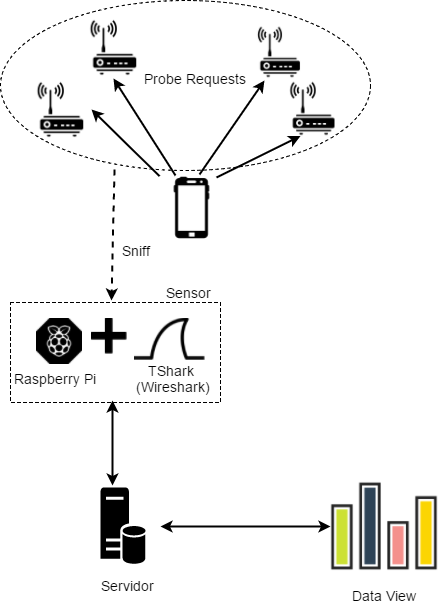
\includegraphics[width=0.50\textwidth]{img/esquema_geral.png}
  \end{center}
  \legend{Fonte: Elaborada pelas autoras.}
\end{figure}

\section{Detalhamento de processos}
O esquema da \autoref{esquema-geral} expõe de maneira mais abstrata o
funcionamento do sistema de medição de tráfego. Já o diagrama de fluxo da
\autoref{diagrama-fluxo} apresenta os processos, entidades externas e
repositórios de armazenamento que compõe o sistema.

\begin{figure}[!h]
  \caption{\label{diagrama-fluxo}Processos e entidades do sistema}
  \begin{center}
    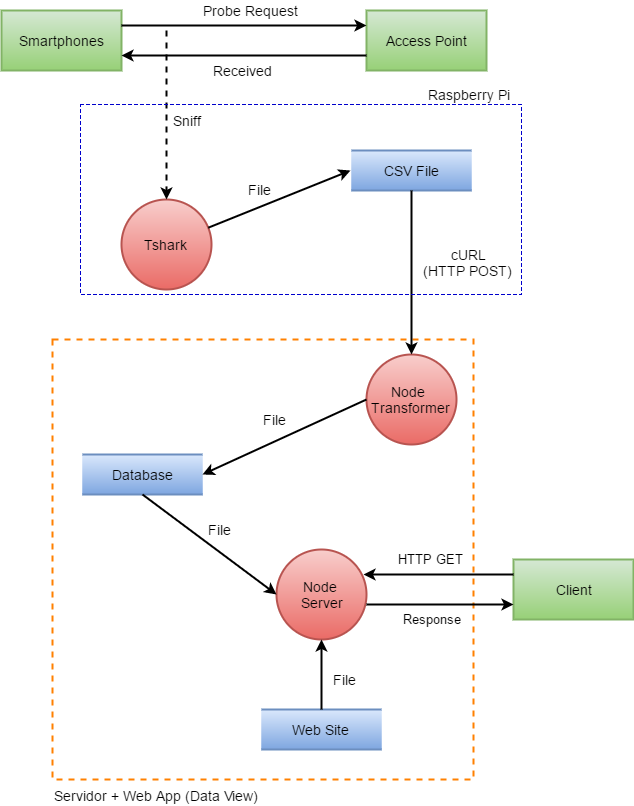
\includegraphics[width=0.70\textwidth]{img/diagrama_fluxo.png}
  \end{center}
  \legend{Fonte: Elaborada pelas autoras.}
\end{figure}

\section{Dispositivo Móvel e \emph{Probe Request}}
\label{smartphone-probe}
Para encontrar redes a que possa se conectar, um dispositivo móvel emite de tempos em tempos (depende da fabricante) pacotes do tipo \emph{probe request} para os APs próximos \cite{Meraki}. Todos os APs que receberem, responderão ao dispositivo (\emph{probe response} ou \emph{received}), então o aparelho descobrirá as redes ao redor disponíveis para conexão.

\section{Sensor}
O sensor é responsável pela detecção de aparelhos e envio de dados ao servidor.

\subsection{Raspberry Pi}
Para a detecção de dispositivos móveis um Raspberry Pi Model 3 B juntamente com um adaptador Wi-Fi são utilizados. O Raspberry foi escolhido,
pois oferece interface amigável de programação (Kali Linux); possui poder de processamento para receber os milhares de pacotes, pré-processá-los
e enviar para o servidor; possui entrada USB pode receber uma antena Wi-Fi e seu tamanho pequeno \cite{rpi2017}.

Outras opções foram consideradas por serem baratas, acessíveis e terem documentação aberta. Foi o caso do ESP8266 que possui um tamanho extremamente
reduzido e possui o custo médio de R\$15,00 \cite{Embarcados2015}, mas seu uso para este trabalho fica impossibilitado. Isso
ocorre, pois essa tecnologia não consegue ser habilitada para o modo monitor da interface de rede \cite{Puhl2016} \cite{Ferreira2016}.

Uma antena Wi-Fi (Ralink MT7601U) foi equipada no Raspberry para ampliar o alcance da captura já que o propósito do sistema é detecção em zonas que podem
apresentar esparcidade de indivíduos (espalhados) e já que ela pôde ser habilitada para o modo monitor (\autoref{modo-monitor}). A antena nativa
do Raspberry não conseguiu ser habilitada para o \emph{monitor mode}.

\subsection{Kali Linux}
O sistema operacional Kali Linux \cite{kali} foi escolhido para o Raspberry Pi, pois possui ampla documentação
para uso em projetos de redes, além de ferramentas, como suporte a drivers de interfaces de rede que possam
ser habilitadas para o modo monitor, foi o caso do Ralink MT7601U.

\subsection{Tshark}
O protocolo Tshark é uma versão de terminal do protocolo
analisador de rede Wireshark \cite{Wireshark2017} \cite{Wireshark2017a}. Ele é
utilizado para analisar e filtrar (\emph{sniff}) e converter os dados dos
pacotes capturados pelo sensor em um arquivo. Esse protocolo foi
escolhido, pois permite realizar o estudo da rede a partir do recebimento de
pacotes e seus campos, além possuir ampla documentação, maturidade e exemplos
por ser uma tecnologia aberta.

\section{Servidor}
O servidor que servirá o Web App será baseado em Node.js. Ele possui duas partes principais que serão apresentadas a seguir.

\subsection{Node Transformer}
\label{node-transformer}
Após converter os dados do pacotes recebidos para um arquivo, o
Raspberry Pi dá um cURL POST (HTTP POST através do terminal) de tempos em tempos
para enviar o arquivo daquela sessão ao servidor. No servidor, o módulo
node transformer particionará o arquivo (segundo alguns campos) em outros
arquivos .JSON que serão salvos no banco de dados.

\subsection{Node Server}
 A partir dos arquivos .JSON citados no item anterior e um Web Site base (HTML,
 CSS, Javascript), o módulo Node Server responde (Response) à requisição do
 cliente (HTTP GET) e apresenta-o os dados capturados.

\section{Data View}
O Data View é a parte do Web App responsável por apresentar os dados capturados
de maneira clara e legível. Para isso, a biblioteca D3.js \cite{D32017} será
utilizada para a plotagem de gráficos a partir dos arquivos .JSON.

\section{Protótipo}
Como apresentação parcial e prova de funcionamento dos componentes anteriores, o protótipo desenvolvido é baseado no sensor.
Trata-se de um Raspberry Pi equipado com um adaptador Wi-Fi que consegue capturar, analisar e exportar os pacotes
\emph{probe request} para um arquivo que será enviado ao servidor. Essa etapa é garantida pelo protocolo de análise de rede
Tshark.

Os comandos do Tshark que capturam os pacotes provenientes dos dispositivos móveis são realizados através de um servidor local
feito em Node.js.

\begin{figure}[!h]
  \caption{\label{prototipo-app}Protótipo do sistema}
  \begin{center}
    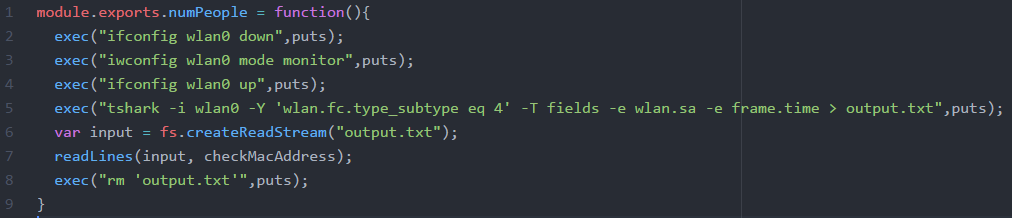
\includegraphics[width=1.0\textwidth]{img/prototipo-app.png}
  \end{center}
  \legend{Fonte: Elaborada pelas autoras.}
\end{figure}

A \autoref{prototipo-app} apresenta o código de um módulo Node.js que
assemelha-se com a função que será desempenhada pelo Node Transformer
(\autoref{node-transformer}). Esse módulo é chamado no servidor. As linhas que
possuem o comando ``exec'' executam comandos diretamente no terminal do sistema
operaciomal. Nas linhas 2-4, habilita-se o adaptador de rede para o modo
monitor. Na linha 5, o comando Tshark rodado representa:

\begin{itemize}
  \item \textbf{wlan0}: interface de rede que indica a antena Wi-Fi;
  \item \textbf{wlan.fc.type\_subtype eq 4}: indica que só pacotes \emph{probe request} devem ser capturados;
  \item \textbf{wlan.sa}: representa o \emph{source address} ou endereço MAC do dispositivo que enviou o pacote;
  \item \textbf{frame.time}: representa a hora, dia e ano em que o pacote foi capturado.
\end{itemize}

Em seguida no código, o arquivo exportado pelo Tshark é lido através de um \emph{stream}. A função ``readLines()''
na linha 7, lê o arquivo linha por linha, identificando os endereços MAC diferentes e adicionando-os a uma lista.
Então, nessa própria função é mostrado no terminal (``console.log(list)''), quantas pessoas foram contadas, ou em outros termos,
quantos dispositivos diferentes foram detectados. Na \autoref{arquivo-pacotes}, mostra-se o arquivo com os pacotes
capturados. Na \autoref{exec-bash} apresenta-se o que a execução da aplicação feita gerou, no caso, detectou
4 pessoas nas proximidades.

\begin{figure}[!h]
  \caption{\label{arquivo-pacotes}Arquivo com pacotes capturados}
  \begin{center}
    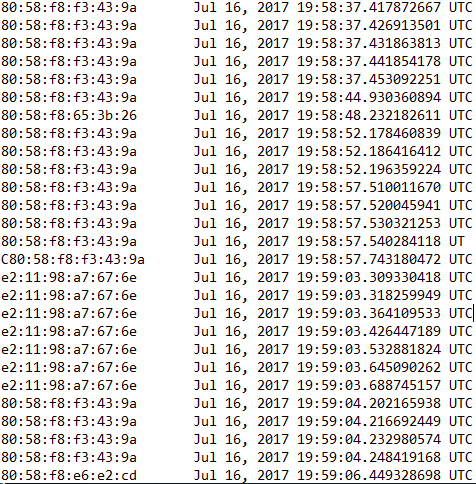
\includegraphics[width=0.70\textwidth]{img/packets.png}
  \end{center}
  \legend{Fonte: Elaborada pelas autoras.}
\end{figure}

\begin{figure}[!h]
  \caption{\label{exec-bash}Resultado da execução da aplicação}
  \begin{center}
    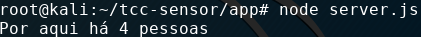
\includegraphics[width=1.0\textwidth]{img/bash.png}
  \end{center}
  \legend{Fonte: Elaborada pelas autoras.}
\end{figure}

\section{Testes e validação do projeto}
Para a validação do sistema proposto serão realizados testes unitários, de integração e
validação. Os testes unitários e de integração do sistema resumem-se em:

\begin{itemize}
  \item detecção dos dispositivos móveis;
  \item comunicação entre Raspberry Pi e servidor;
  \item comunicação servidor e interface;
  \item processamento de dados capturados em dados desejados;
  \item determinar se sistema consegue contar pessoas.
\end{itemize}

Já os testes de validação são resumidos em determinar se o sistema consegue ou
não determinar a contagem e o tráfego de pessoas. Para tanto, serão feitos testes em
ambientes controlados e não controlados. Os controlados são
aquelas zonas em que sabe-se o número de pessoas, e então confere-se com o resultante da
detecção. Nos ambientes não-controlados, o tráfego de pessoas será testado.

A taxa de confiabilidade no sistema será baseada no desvio padrão dos testes
realizados em ambiente controlados.
O sistema final vai ser considerado aplicável ou não caso o desvio
padrão determinado fique dentro
dos limites estabelecidos.

Inicialmente, visa-se desenvolver os primeiros testes em ambiente
controlado, numa área pequena e com poucos dispositivos móveis, para verificar o
comportamento do sistema desenvolvido na medição do tráfego. Após testes
iniciais, pretende-se encontrar uma organização parceira que esteja dentro das
especificações necessárias e deseje conhecer melhor seu público alvo, cedendo
seu espaço e sua rede para alguns procedimentos e testes com a aplicação proposta
 - nessa etapa, o projeto busca verificar o desempenho do
sistema em ambiente real, com maior quantidade de dispositivos móveis.

\section{Análise de Riscos}
Considerando as premissas dos tópicos anteriores, há alguns itens e áreas que podem sofrer desvios ao longo do trabalho. Estes itens e seus planos
de contingência respectivamente são:

\begin{itemize}
  \item Falha da detecção de dispositivos (precisão): serão feitas duas formas de detecção através do protocolo Tshark, as duas garantem que os dados
  de uma e outra são verídicos, caso uma falhe há a outra para detectar os aparelhos móveis;
  \item Processamento no servidor é complexa: caso o desenvolvimento do processamento de dados no servidor seja muito complexa e considerando
  que trabalharemos com estatísticas, optar por uma \emph{cloud} seria uma opção;
  \item Raspberry Pi perder a conexão com a rede para mandar dados ao servidor: um backup dos dados será feito no aparelho, e então quando
  a conexão retornar, esses serão enviado ao servidor. Também há a possibilidade do uso de um Modem 3G para garantir o envio.
\end{itemize}
 % inclui o arquivo metodologia.tex

\chapter{Cronograma}
\label{cronograma}

Teste.


\chapter{Conclusão}
\label{conclusao}

O foco principal deste trabalho foi disponibilizar um sistema \emph{opensource}
que aplique os conceitos de \emph{geomarketing} vistos, abrangendo o estudo de
redes de computadores (redes sem fio) e dispositivos móveis aplicados à
administração, com ênfase em gestão da informação. A partir conceitos de
\emph{geomarketing} provenientes de autores, consultorias e trabalhos
semelhantes, foi possível agrupar a contagem de pessoas por períodos e descobrir
informações relevantes para a tomada de decisão estratégica em negócios
(\autoref{importancia}).

Salientamos que, como a as soluções de \emph{geomarketing}
são, em maior parte, de âmbito privado, grande parte da fundamentação teórica
volta-se para consultorias, estudos de caso e trabalhos correlatos. Por essa
razão, não foi possível o levantamento de dados financeiros sobre custos do serviço. Em livros, muitos conceitos teóricos podem ser encontrados -
entretanto, não como são aplicados, existiram dificuldades no desenvolvimento do
sistema proposto, como decidir de que forma organizar a fase estatística na
agregação/ contagem de pessoas e processamento de dados: a precisão do sistema e
as informações coletadas devem ser relevantes e numerosas (generalização).

O sistema desenvolvido consegue realizar a contagem de pessoas em zonas
específicas, porém ressalvamos que, em áreas muito grandes, faz-se necessário
multiplicar o número de sensores de acordo com a cobertura necessitada, a fim de
manter-se resultados pontuais.

Outro fator é que, no experimento realizado no LTIA, a diferença entre o número
real de pessoas e o detectado foi grande:  observou-se que, em locais com alta
de densidade de máquinas e dispositivos fixos por pessoa, a eficácia da
estimativa é comprometida: como a quantia de dispositivos é muito mais alta do
que a de pessoas, esse fator pode inflar as estimativas, exibindo uma frequência
de pessoas acima do real. Logo, por se basear no \emph{MAC Address} de
dispositivos para contagem, o sistema não é indicado para medição em locais com
alta concentração de aparelhos fixos.

O contator se comporta bem em áreas onde existe alta frequência na entrada e saída de pessoas, como
restaurantes e lojas, em que os transeuntes geralmente portam um aparelho móvel
pessoal (\emph{smarthphone} ou \emph{tablet}). Portanto, o dispositivo não é indicado para espaços com poucas pessoas e muita quantidade de máquinas ao redor. O GSmart seria bastante útil na gestão de rede e dimensionamento de perfil tecnológico, por exemplo.

Foi observado também que, indivíduos inicialmente detectados no ambiente, ao irem embora, ainda permanecerão na contagem, ou seja: a saída de pessoas não é considerada, somente a chegada - se uma pessoa ficar por apenas 1 minuto no local, será contada pelo dispositivo. Para futura implementação, seria interessante capturar também o tempo de permanência de cada indivíduo/ MAC na área, além de utilizar esse período para validar se, por exemplo, uma pessoa que adentre um estabelecimento comercial de fato utilizou os serviços do local ou se está somente de passagem. Durante o tempo de detecção, ocorrem intervalos em que pessoas podem não ser detectadas, causados por interferências, obstáculos ou limitações tecnológicas, conforme descrito na \autoref{wifi} e \autoref{erros-influencia}.

Diante do exposto neste trabalho, apesar das limitações verificadas, concluímos
que o dispositivo cumpre o objetivo de medição de tráfego com baixa exatidão e precisão média,
além de prover
estatísticas comparativas e métricas. Além disso, o GSMART mostrou-se uma
ferramenta muito útil para estudantes, proporcionando recursos ao estudo de
\emph{geomarketing} à comunidade aberta e demais interessados.


\section{Trabalhos Futuros}
Como trabalhos futuros, propõe-se alguma melhorias para garantir maior exatidão e
precisão do sistema deste trabalho. Essas melhorias são:
\begin{itemize}
    \item \textbf{Tempo de estadia}: considerar um tempo mínimo de estadia dentro de uma zona para indivíduo ser
    contado;
    \item \textbf{Classificar dispositivos}: tentar diferenciar \emph{smartphones} de computadores comerciais;
    \item \textbf{Explorar comunicação GSM}: com autorização de empresas de telefonia, explorar comunicação GSM
    para não depender somente do Wi-Fi;
    \item \textbf{Detectar múltiplos aparelhos por pessoa}: através da potência de sinal e \emph{timestamp}
    de pacotes determinar se dispositivos tendem a pertencer a um mesmo indivíduo.
\end{itemize}

Além da melhoria no trabalho desenvolvido, indica-se o sistema construído como um potencial para gestão de redes
de computadores dentro de zonas urbanas e rurais onde é possível mapear grande quantidade de dispositivos com o
que já foi levantado neste trabalho. Além disso, pode-se aplicar o GSMART como ferramenta de decisões para mobilidade
urbana a partir do momento em que horas de pico de tráfego podem ser inferidas.
 % inclui o arquivo conclusao.tex

% ----------------------------------------------------------
% ELEMENTOS PÓS-TEXTUAIS
% ----------------------------------------------------------

% ----------------------------------------------------------
% Referências bibliográficas
% ----------------------------------------------------------
\bibliography{referencias}
% ----------------------------------------------------------

\end{document}
